% !TEX encoding = UTF-8
% !TEX TS-program = pdflatex
% !TEX root = ../tesi.tex

%**************************************************************
\chapter{Verifica e validazione}
\label{cap:verifica-validazione}
%**************************************************************
\intro{In questo capitolo si descrivono i processi di verifica e validazione del prodotto, descrivendo i tool utilizzati per valutare il corretto funzionamento e la qualità del prodotto.} 
	\section{Verifica}
		Vengono di seguito descritti gli strumenti utilizzati per verificare la correttezza di tutto il materiale prodotto durante lo stage.
		\subsection{Documentazione}
			Durante lo stage c'è stata la necessità della stesura di alcuni documenti quali:
			\begin{itemize}
				\item Analisi dei Requisiti: documento mirato a riassumere i requisiti dello stage e individuare i casi d'uso del progetto;
				\item Progettazione Tecnica: documento mirato a definire una struttura generica dalla quale partire per lo sviluppo nella fase di codifica;
				\item Manuale Installazione: manuale contenente una guida testuale all'installazione del prodotto e al suo uso (come per esempio la gestione dei file XML);
				\item Manuale Manutenzione: manuale contenente una descrizione generica di come è implementato/strutturato il progetto, nel quale si vanno a spiegare potenziali punti di estensione e, se ci sono, eventuali problemi  presenti nel codice.
			\end{itemize}
			Per la redazione di tali documenti è stato usato \LaTeX, i cui file sorgenti son stati verificati tramite Spell Checker, estensione di VsCode per la verifica di errori ortografici all'interno di file sorgenti, permettendo come dizionari sia quello italiano che quello inglese.\\
			
		\subsection{Codice}
			Per quanto non fosse un requisito dello stage, durante la codifica, alcune parti del codice hanno richiesto la stesura di test di unità. \\
			Questo perché, per quanto il codice sia stato scritto seguendo il maggior numero di best practice possibile, ci son state parti particolarmente algoritmiche intrinsecamente poco leggibili. Per questo motivo son stati sviluppati dei test di unità automatici che vanno a verificare i requisiti che i metodi di queste classi devono rispettare, così da semplificare la manutenzione e modifica futura di tale codice. \\
			Per la redazione di tali test è stato usato \texttt{JUnit4}, libreria Java per appunto lo sviluppo di suite di test di unità.
			\begin{center}
				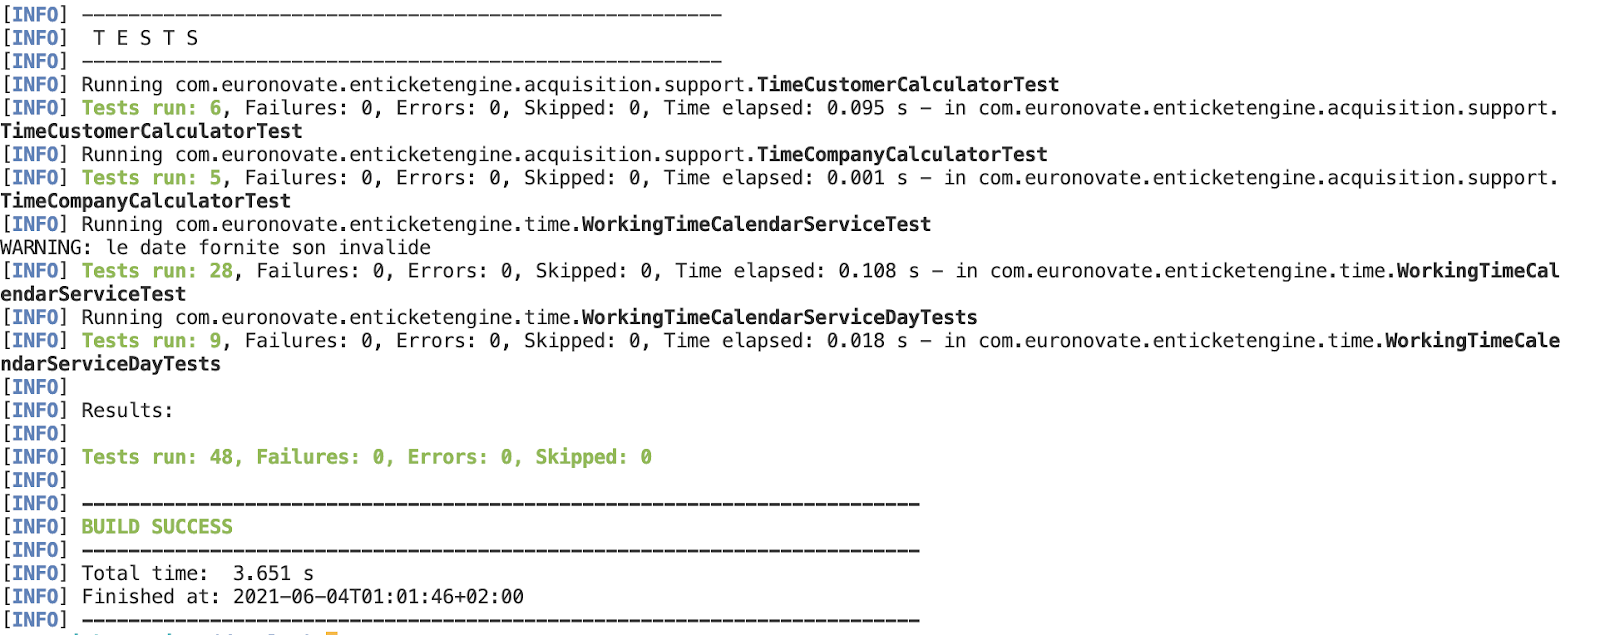
\includegraphics[keepaspectratio = true, width=16cm]{immagini/test.png}
				\captionof{figure}{Report suite test di unità}
			\end{center}
	\section{Validazione}
		Viene di seguito descritto il processo di validazione del materiale prodotto durante il periodo di stage.
		\subsection{Documentazione}
			La validazione  della documentazione prodotta durante lo stage è stata effettuata dal tutor aziendale Matteo Gnoato, assumendo il ruolo di committente: egli stabiliva se la documentazione fosse conforme e corretta rispetto a quanto atteso e, dopo aver chiesto delle eventuali correzioni, il documento veniva approvato e inviato a tutte le persone coinvolte ed interessate in questo progetto di stage.
		\subsection{Codice}
			La validazione del codice è avvenuta in due fasi.\\
			La prima, ufficiosa, è avvenuta con il tutor aziendale in meeting privati, nel quale si andava a ispezionare il codice per verificarne tutte le proprietà richieste, come leggibilità, testabilità, manutenibilità e correttezza. \\
			La seconda, ufficiale, l'ultimo giorno del progetto di stage, il giorno 10 Giugno 2021, con una demo, il cui scopo è stato quello di mostrare all'azienda ciò che si ha realizzato durante il periodo di stage, al fine di determinare il grado di soddisfazione dei requisiti stabiliti. Tale demo è avvenuta da remoto, con presenti il tutor aziendale e alcuni dipendenti di Euronovate che hanno partecipato all'individuazione dei requisiti (Quality Assurance) e al deploy dell'applicativo finale. \\
			